% Appendix Template

\newcommand{\major}{2}
\newcommand{\minor}{3}

\newcommand{\undPrefix}{\major_\minor}
\newcommand{\dotPrefix}{\major.\minor}
\newcommand{\scoPrefix}{\major-\minor}
\newcommand{\filePrefix}{\undPrefix}

\chapter{Results of experiment \dotPrefix} % Main appendix title


\label{Appendix\scoPrefix} % Change X to a consecutive letter; for referencing this appendix elsewhere, use \ref{AppendixX}
These experiments are discussed \hyperref[disc:h2]{here}

\begin{figure}[ht]
  \centering
  \begin{subfigure}[t]{0.5\linewidth}
    \centering\captionsetup{width=.8\linewidth}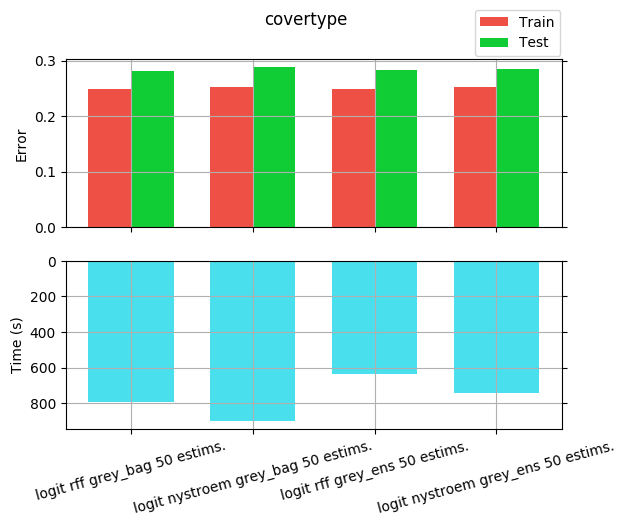
\includegraphics[width=\imgscale\linewidth]{Figures/\filePrefix/covertype}
    \caption{Exp 2.3 with Covertype. Error is decreased by 10\% approx.}
    \label{fig:\undPrefix_covertype}
  \end{subfigure}%
  \begin{subfigure}[t]{0.5\linewidth}
    \centering\captionsetup{width=.8\linewidth}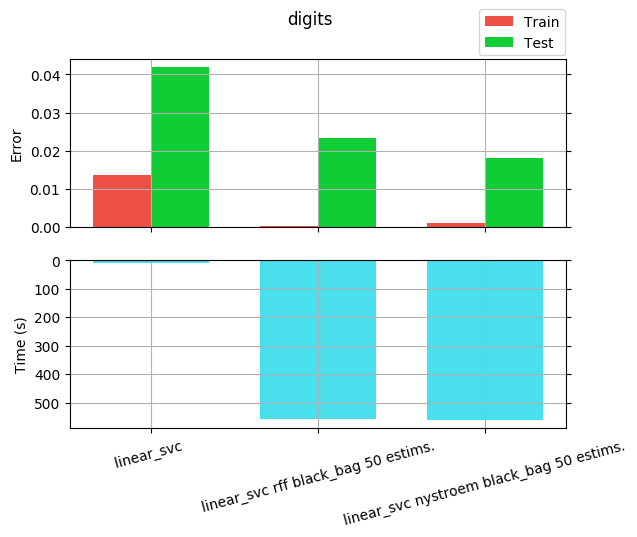
\includegraphics[width=\imgscale\linewidth]{Figures/\filePrefix/digits}
    \caption{Exp 2.3 with Digits. Error is decreased by 2\% approx.}
    \label{fig:\undPrefix_digits}
  \end{subfigure}
\end{figure}


\begin{figure}[ht]
  \centering
  \begin{subfigure}[t]{0.5\linewidth}
    \centering\captionsetup{width=.8\linewidth}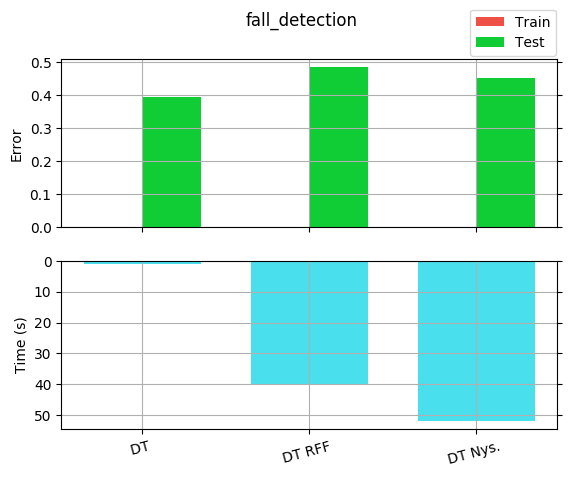
\includegraphics[width=\imgscale\linewidth]{Figures/\filePrefix/fall_detection}
    \caption{Exp 2.3 with Fall Detection. Error is not decreased.}
    \label{fig:\undPrefix_fall_detection}
  \end{subfigure}%
  \begin{subfigure}[t]{0.5\linewidth}
    \centering\captionsetup{width=.8\linewidth}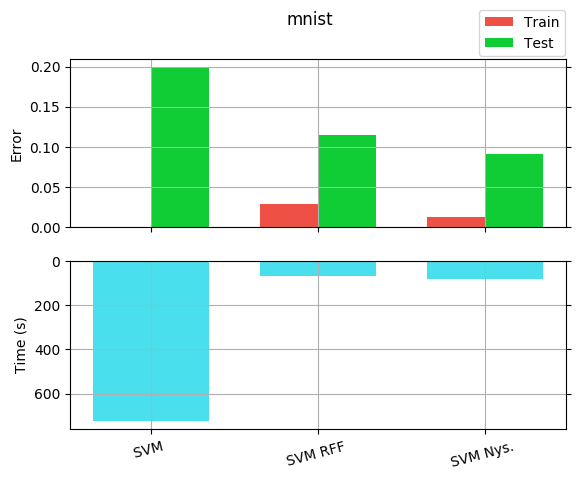
\includegraphics[width=\imgscale\linewidth]{Figures/\filePrefix/mnist}
    \caption{Exp 2.3 with MNIST. Error is decreased by 10\% approx.}
    \label{fig:\undPrefix_mnist}
  \end{subfigure}
\end{figure}


\begin{figure}[ht]
  \centering
  \begin{subfigure}[t]{0.5\linewidth}
    \centering\captionsetup{width=.8\linewidth}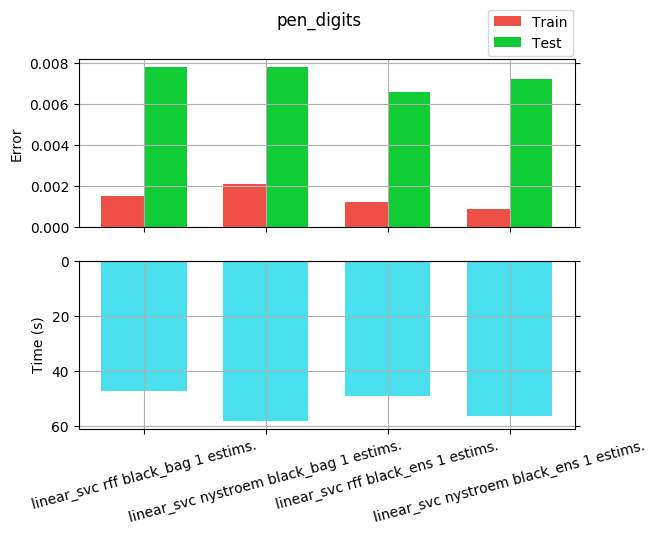
\includegraphics[width=\imgscale\linewidth]{Figures/\filePrefix/pen_digits}
    \caption{Exp 2.3 with Pen Digits. Error is decreased by 5\% approx.}
    \label{fig:\undPrefix_pen_digits}
  \end{subfigure}%
  \begin{subfigure}[t]{0.5\linewidth}
    \centering\captionsetup{width=.8\linewidth}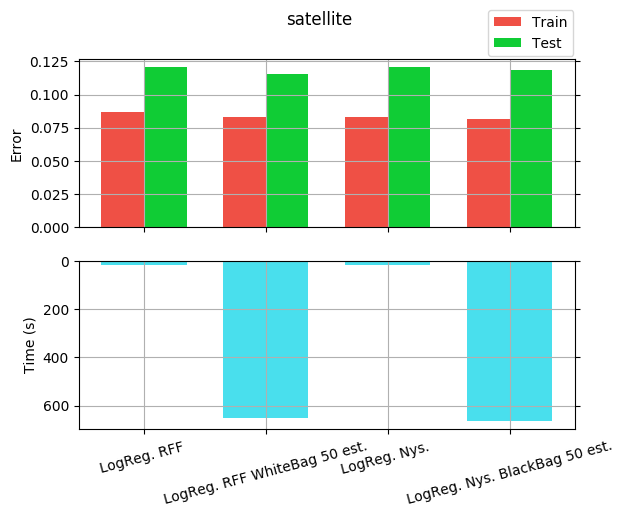
\includegraphics[width=\imgscale\linewidth]{Figures/\filePrefix/satellite}
    \caption{Exp 2.3 with Satellite. Error is decreased by 7\% approx.}
    \label{fig:\undPrefix_satellite}
  \end{subfigure}
\end{figure}

\begin{figure}[ht]
  \centering
  \begin{subfigure}[t]{0.5\linewidth}
    \centering\captionsetup{width=.8\linewidth}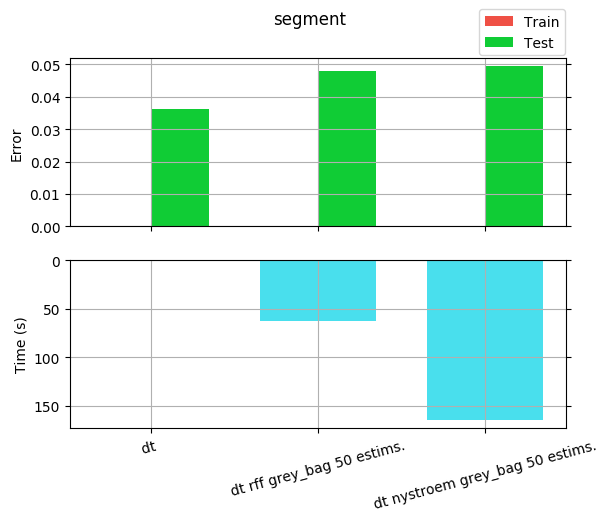
\includegraphics[width=\imgscale\linewidth]{Figures/\filePrefix/segment}
    \caption{Exp 2.3 with Segment. Error is decreased by 2\% approx.}
    \label{fig:\undPrefix_segment}
  \end{subfigure}%
  \begin{subfigure}[t]{0.5\linewidth}
    \centering\captionsetup{width=.8\linewidth}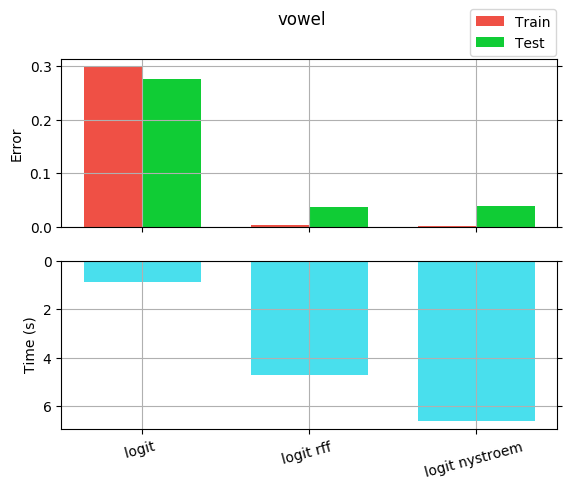
\includegraphics[width=\imgscale\linewidth]{Figures/\filePrefix/vowel}
    \caption{Exp 2.3 with Vowel. Error is decreased by 35\% approx.}
    \label{fig:\undPrefix_vowel}
  \end{subfigure}
\end{figure}



\begin{figure}[ht]
  \centering
  \begin{subfigure}[t]{0.5\linewidth}
    \centering\captionsetup{width=.8\linewidth}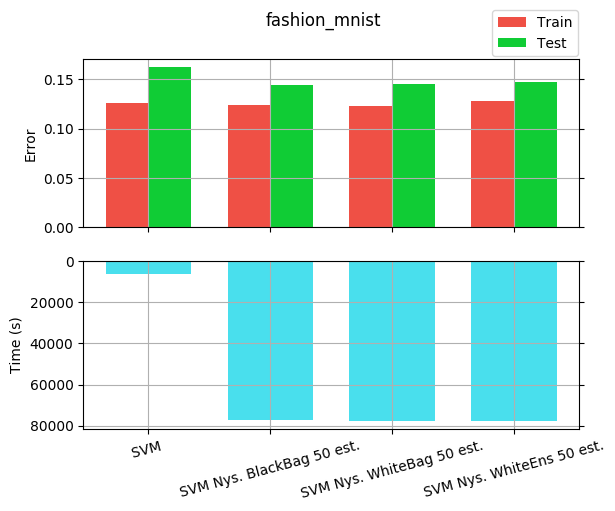
\includegraphics[width=\imgscale\linewidth]{Figures/\filePrefix/fashion_mnist}
    \caption{Exp 2.3 with Fashion MNIST. Error is decreased by 2\% approx.}
    \label{fig:\undPrefix_segment}
  \end{subfigure}%
\end{figure}


\let\major\undefined
\let\minor\undefined

\let\undPrefix\undefined
\let\dotPrefix\undefined
\let\scoPrefix\undefined

\let\filePrefix\undefined
